\section{Implementazione della FFT e la sua simulazione}

\noindent Una volta verificato il funzionamento dell'unità butterfly, si è implementata la struttura per la FFT, come nell'immagine sottostante.
\noindent \begin{figure}[H]
      \centering
      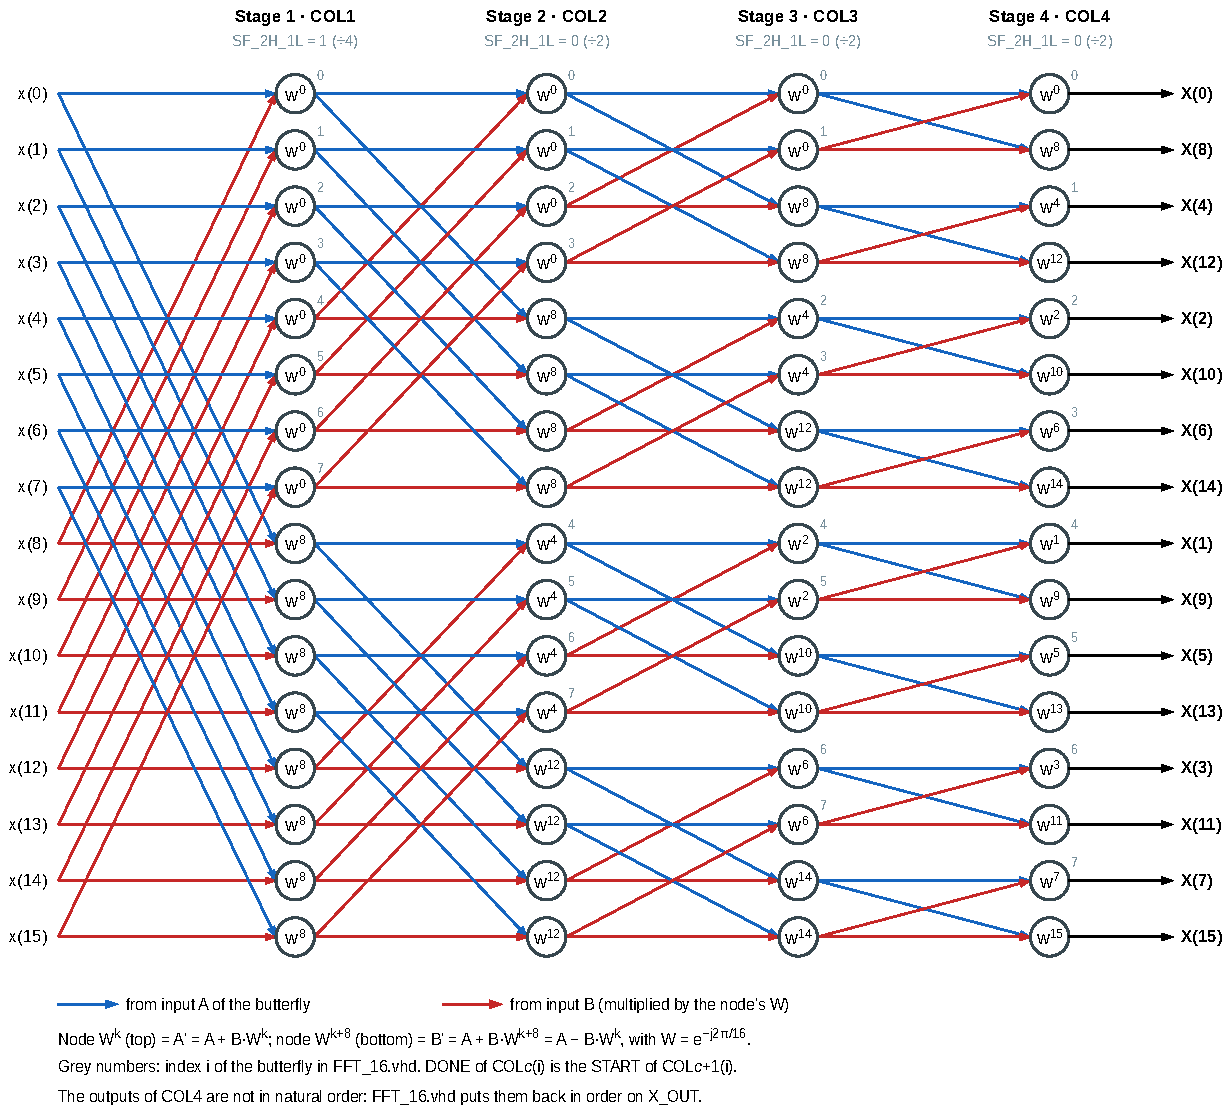
\includegraphics[width=1\textwidth]{fig10_fft16}
      \caption{Schema FFT realizzato}
\end{figure}

\noindent Lo schema evidenzia quattro colonne da 8 butterfly ciascuna, ossia quattro stadi di calcolo, per un totale di 32 butterfly necessarie per compiere una FFT.

\noindent Nel primo stadio, si connettono nodi separati di una quantità pari ad otto, ossia si collegano x(0) e x(8), x(1) e x(9) e così via. Si imposta, inoltre, come da specifica, che solo in tale stadio SF\_2H\_1L sia alto, per gestire l'overflow iniziale di due bit. Negli stadi successivi, invece, è richiesto che SF\_2H\_1L  sia basso. Poiché il numero totale di shift verso destra effettuati sui dati elaborati è pari a 5 (due al primo stadio, uno in tutti gli altri), ci si aspetta uno scale factor di $2^5 = 32$ sui dati di uscita, ovvero che le uscite ottenute dovranno essere implicitamente moltiplicate per tale quantità, al fine di ottenere i risultati correttamente scalati.

\noindent Superato il primo stadio, il sistema organizza i dati separando i percorsi degli stessi in due sottoinsiemi: le uscite A vengono accoppiate tra loro ed elaborate assieme nelle butterfly della colonna successiva, così come le B. In questo modo, si riesce a dividere il problema originale in due blocchi più piccoli e indipendenti, permettendo agli stadi seguenti di lavorare su sotto-insiemi di dati intermedi più piccoli. Di conseguenza, il numero di sottoinsiemi raddoppia dopo ogni stadio.
In aggiunta, escludendo il primo stadio, i coefficienti W variano tra le varie unità butterfly di una singola colonna. L'ultimo stadio, che collega nodi adiacenti, presenta la massima variabilità dei valori W, dato che ad ogni butterfly è associato un coefficiente di rotazione differente.

\noindent Il file VHDL "FFT\_16" che descrive questa architettura e i collegamenti tra le unità è disponibile nella cartella \texttt{rtl/} della repository. A ciascuna butterfly è stato fornito lo stesso reset asincrono e lo stesso reset sincrono, i quali arrivano dall'esterno; inoltre, è stato inchiodato per ciascuna di esse il segnale SF\_2H\_1L. Al fine di presentare un file più rifinito, si sono definiti dei segnali WR e WI al fine di poter raggruppare i portmap delle unità.
\noindent La testbench della FFT (TB\_FFT\_16, nella cartella \texttt{tb/} della repository) è divisa in due parti. Nella prima si applicano i 6 vettori di test forniti dal docente, i cui risultati sono riportati di seguito; nella seconda si eseguono alcuni test aggiuntivi, ad esempio con ingressi complessi e con l'attivazione del reset sincrono durante un'elaborazione, al fine di verificare il corretto funzionamento dell'architettura anche in questi casi.

\noindent Si procede ora a testare la trasformata di Fourier tramite i 6 vettori di test forniti dal docente, i quali risultano sufficienti a verificarne il comportamento, grazie alla variabilità degli stessi. I dati ottenuti dalle simulazioni risultano compatibili con quanto previsto teoricamente. Di seguito, si allegano i vettori utilizzati per la simulazione della FFT, tenendo conto che, ai fini del testing, si sono considerate unicamente le prime 9 componenti dell'uscita. Nella tabella successiva, si presentano i vettori di test utilizzati, sottolineando che le componenti sono indicate dalla posizione 0 alla 15 in ordine crescente.

\begin{table}[H]
    \centering
    \begin{tabular}{|c|l|}
        \hline
        \textbf{Numero Identificativo} & \textbf{Vettore di Test [0 - 15]} \\
        \hline
        1 & [-1,-1,-1,-1,-1,-1,-1,-1,-1,-1,-1,-1,-1,-1,-1,-1] \\
        \hline
        2 & [-1,0,1,0,-1,0,1,0,-1,0,1,0,-1,0,1,0] \\
        \hline
        3 & [1,0,0,0,0,0,0,0,0,0,0,0,0,0,0,0] \\
        \hline
        4 & [-1,-1,+1,+1,-1,-1,+1,+1,-1,-1,+1,+1,-1,-1,+1,+1] \\
        \hline
        5 & [0.5,0.5,0.5,0.5,0.5,0.5,0.5,0.5,0.5,-0.5,-0.5,-0.5,-0.5,-0.5,-0.5,-0.5] \\
        \hline
        6 & [0,0,0,0,0,0,0,0,0.75,0,0,0,0,0,0,0] \\
        \hline
    \end{tabular}
        \caption{Vettori di test utilizzati per la simulazione}
    \label{tab:vettori_test}
\end{table}

\begin{comment}
\begin{itemize}
    \item \textbf{Test 1: DC Costante (Segnale Continuo)}
    \begin{itemize}
        \item \textbf{Ingresso:} Tutti i 16 campioni fissati a $x[n] = -1.0$ (\texttt{1000...0}).
        \item \textbf{Analisi:} Segnale puramente stazionario; l'energia si concentra nel bin a frequenza zero.
        \item \textbf{Uscita attesa:} 
        \begin{itemize}
            \item Bin $k=0$: Parte reale negativo pari a $-16$ (in formato Q1.23).
            \item Bin $k=1 \dots 15$: Parte reale nulla.
            \item Per tutti i bit: parte immaginaria nulla.
        \end{itemize}
    \end{itemize}

    \item \textbf{Test 2: Onda Sinusoidale Pura} 
    \begin{itemize}
        \item \textbf{Ingresso:} Sequenza periodica $\{0, 1, 0, -1\}$ con periodo pari a $T=4$ campioni.
        \item \textbf{Analisi:} Corrisponde a una sinusoide digitale con frequenza $f = f_s/4$.
        \item \textbf{Uscita attesa:}
        \begin{itemize}
            \item Bit $k=4$ e $k=12$: Picchi di ampiezza puramente immaginaria (frequenza positiva e negativa).
            \item Altri Bit: Valori nulli.
        \end{itemize}
    \end{itemize}

    \item \textbf{Test 3: Impulso Delta Finale} 
    \begin{itemize}
        \item \textbf{Ingresso:} $\delta[n-15]$ (tutti 0 tranne l'ultimo campione pari a $\approx 1.0$).
        \item \textbf{Analisi:} La trasformata di un impulso ritardato ha modulo costante e fase linearmente decrescente.
        \item \textbf{Uscita attesa:}
        \begin{itemize}
            \item Parte reale: Costante per ogni $k$ (valore reale circa $1/32 \approx 0.031$).
            \item Fase: I valori complessi ruotano nel piano di Gauss seguendo l'esponenziale $e^{-j\frac{2\pi}{16}15k}$.
        \end{itemize}
    \end{itemize}

    \item \textbf{Test 4: Onda Quadra (Periodo 4)} 
    \begin{itemize}
        \item \textbf{Ingresso:} Sequenza $\{+1, +1, -1, -1\}$ ripetuta.
        \item \textbf{Analisi:} Simile al test 2, ma con forma d'onda quadra. La componente fondamentale è a $k=4$.
        \item \textbf{Uscita attesa:}
        \begin{itemize}
            \item Bin $k=4, 12$: Picchi principali nella parte reale/complessa a seconda della fase iniziale.
            \item Armoniche superiori: Generalmente nulle o ripiegate (aliasing) a causa della bassa frequenza di campionamento rispetto al segnale.
        \end{itemize}
    \end{itemize}

    \item \textbf{Test 5: Onda Rettangolare Lunga} 
    \begin{itemize}
        \item \textbf{Ingresso:} Segnale asimmetrico (9 campioni a $+0.5$ e 7 campioni a $-0.5$).
        \item \textbf{Analisi:} Il segnale ha una componente DC non nulla e una fondamentale a $k=1$.
        \item \textbf{Uscita attesa:}
        \begin{itemize}
            \item Bin $k=0$: Piccola componente reale positiva (valore netto $1.0/32$).
            \item Bin $k=1, 15$: Picchi principali (fondamentale).
            \item Bin dispari ($3, 5, \dots$): Armoniche decrescenti tipiche dell'onda quadra.
        \end{itemize}
    \end{itemize}

    \item \textbf{Test 6: Impulso Delta Centrale} 
    \begin{itemize}
        \item \textbf{Ingresso:} $\delta[n-8]$ (impulso pari a $0.75$ esattamente a metà finestra).
        \item \textbf{Analisi:} Lo spostamento di $N/2$ nel tempo produce una fase alternata $(-1)^k$.
        \item \textbf{Uscita attesa:}
        \begin{itemize}
            \item Parte Reale: Valori che alternano segno tra bin pari e bin dispari.
            \item Parte Immaginaria: Nulla (poiché l'impulso è sull'asse di simmetria reale).
            \item Ampiezza: Modulo costante pari a $0.75 \times 0.5 = 0.375$ (scalato).
        \end{itemize}
    \end{itemize}
\end{itemize}
\end{comment}

\begin{figure}[H]
      \centering
      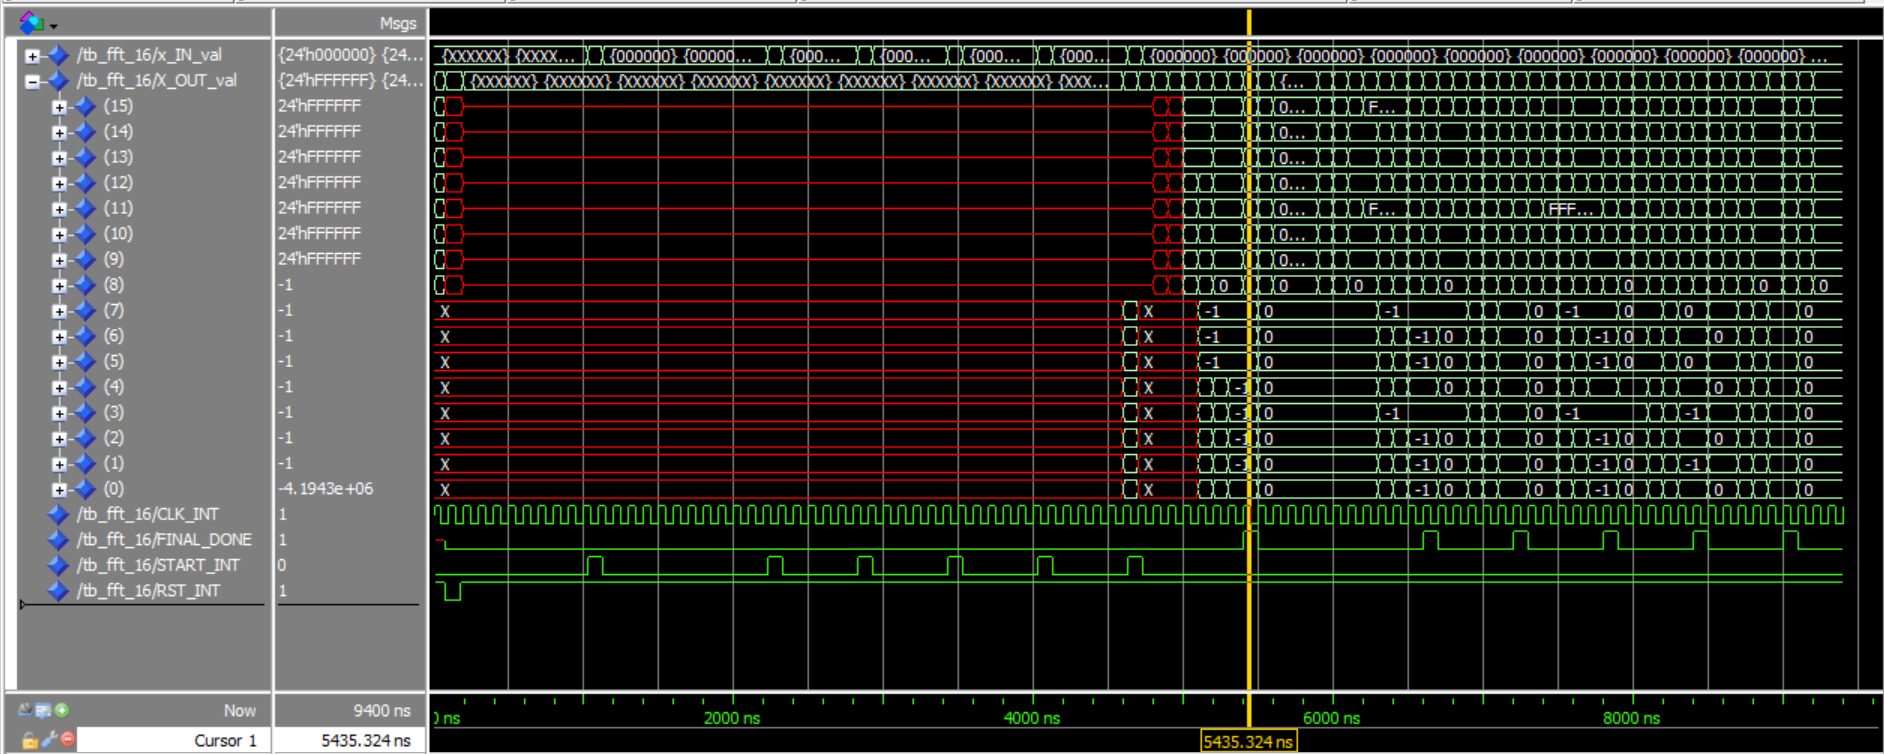
\includegraphics[width=1\textwidth]{sim_tb_fft_16}
      \caption{Schermata della simulazione completa, con focus sulle parti reali dei risultati del test 1}
\end{figure}
\begin{figure}[H]
      \centering
      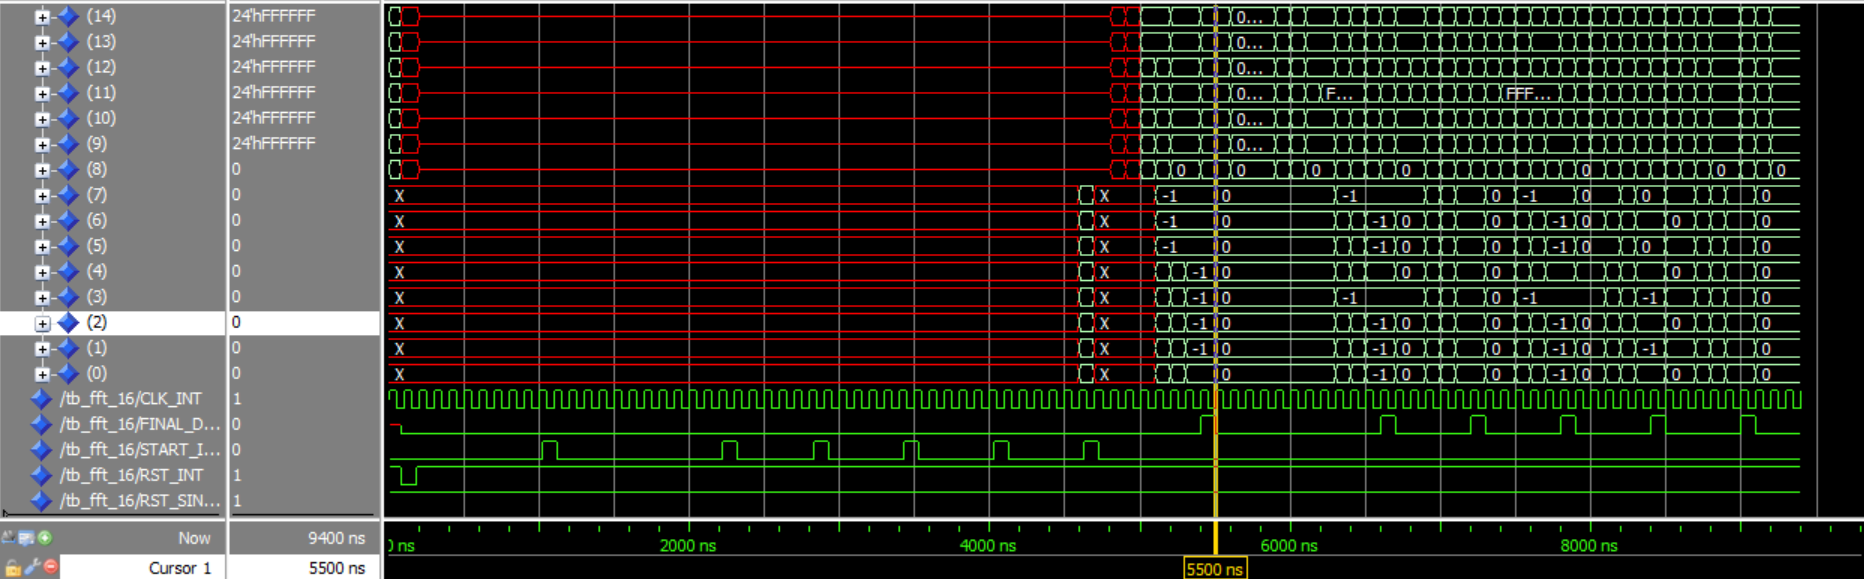
\includegraphics[width=1\textwidth]{sim_test1_imag}
      \caption{Schermata della simulazione completa, con focus sulle parti immaginarie dei risultati del test 1}
\end{figure}
\begin{figure}[H]
      \centering
      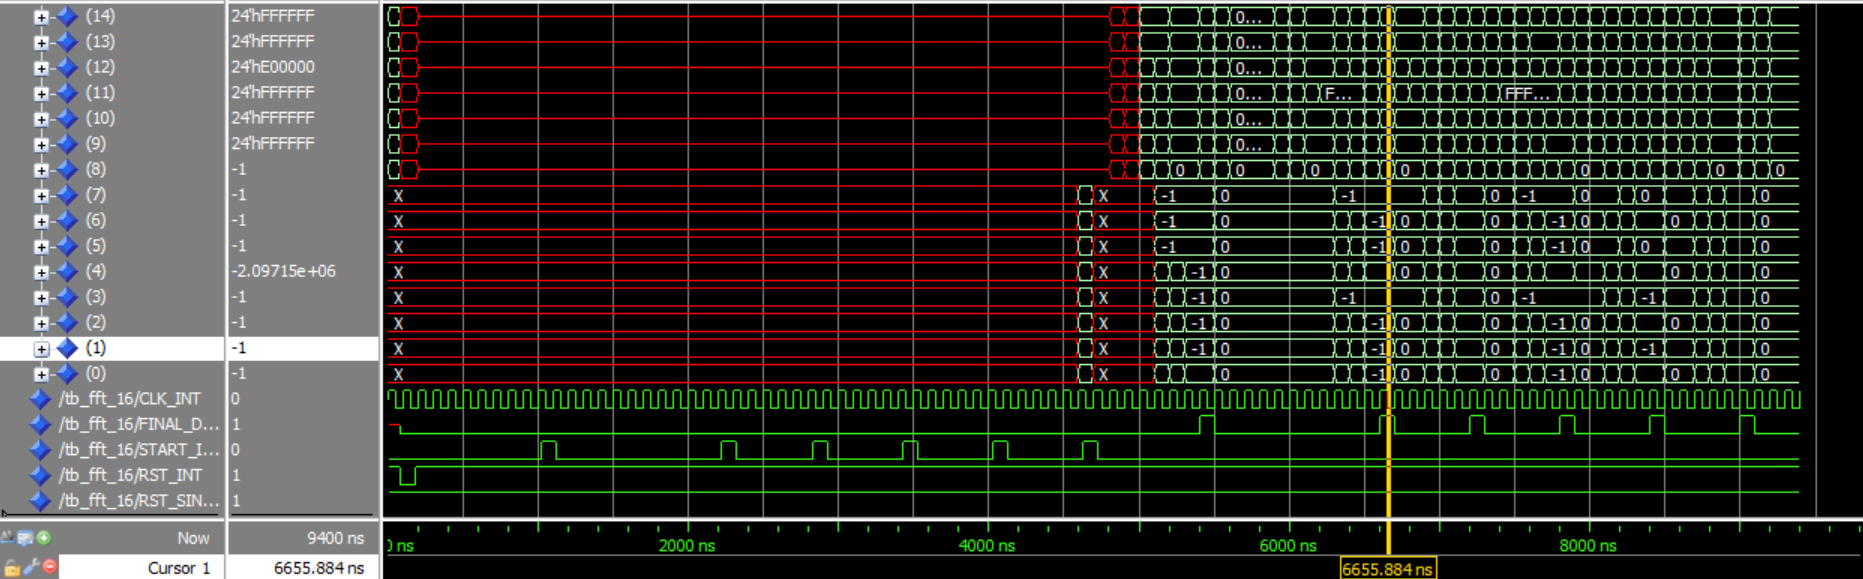
\includegraphics[width=1\textwidth]{sim_test2_real}
      \caption{Schermata della simulazione completa, con focus sulle parti reali dei risultati del test 2}
\end{figure}
\begin{figure}[H]
      \centering
      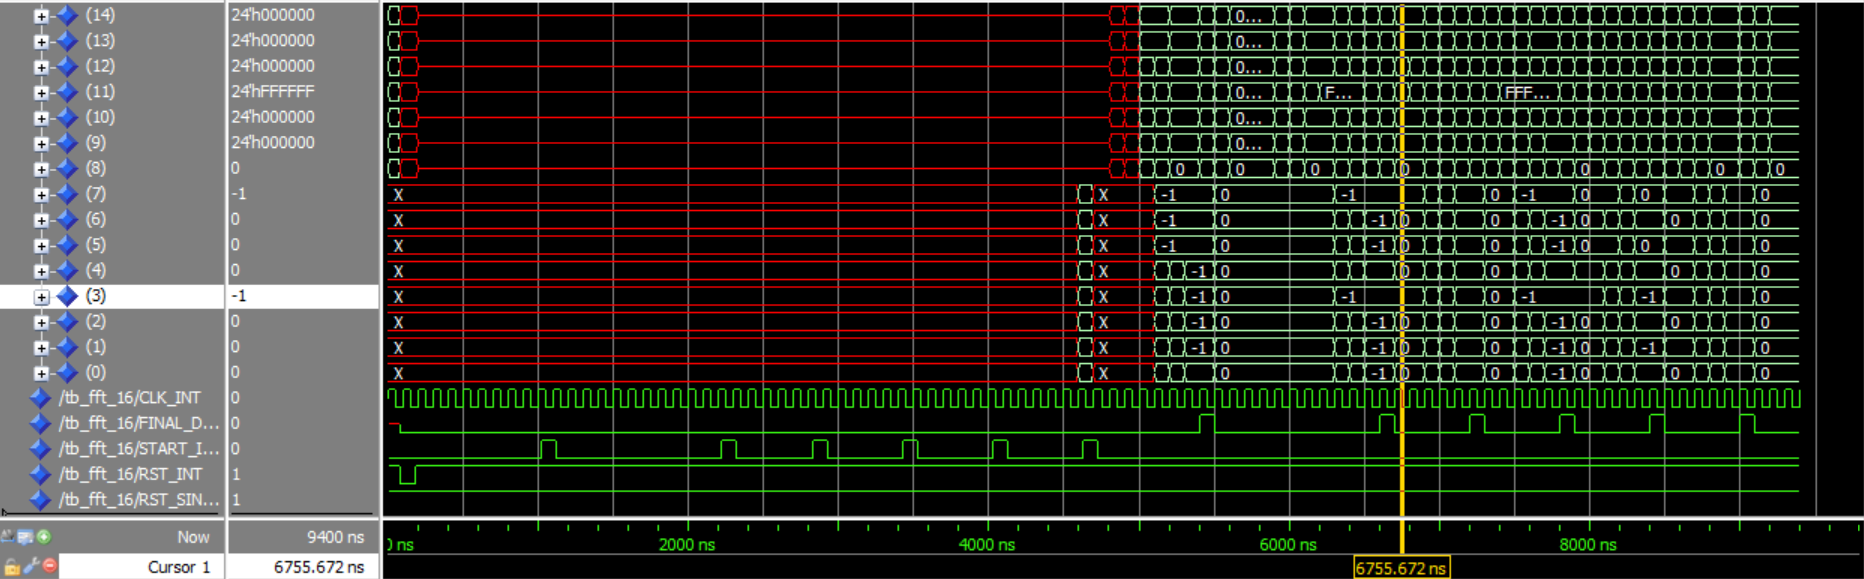
\includegraphics[width=1\textwidth]{sim_test2_imag}
      \caption{Schermata della simulazione completa, con focus sulle parti immaginarie dei risultati del test 2}
\end{figure}
\begin{figure}[H]
      \centering
      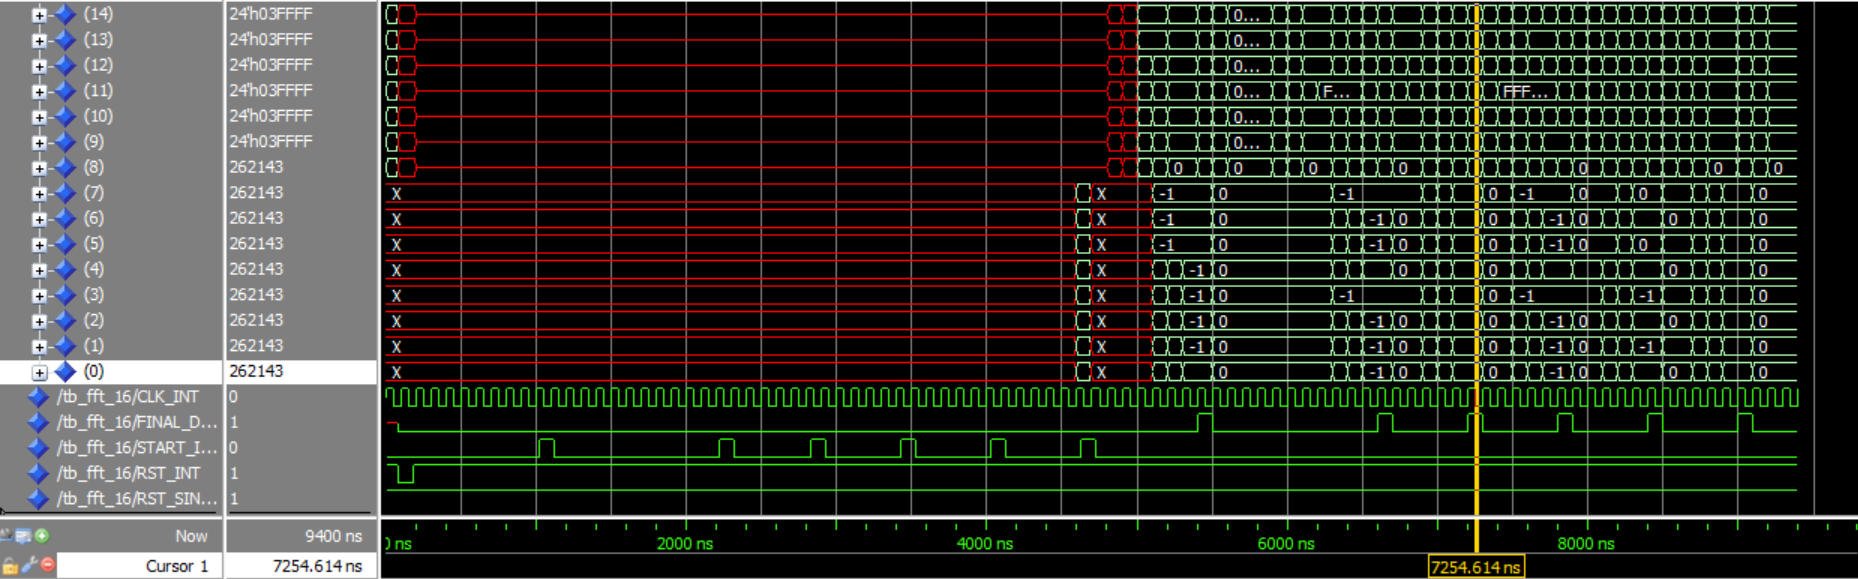
\includegraphics[width=1\textwidth]{sim_test3_real}
      \caption{Schermata della simulazione completa, con focus sulle parti reali dei risultati del test 3}
\end{figure}
\begin{figure}[H]
      \centering
      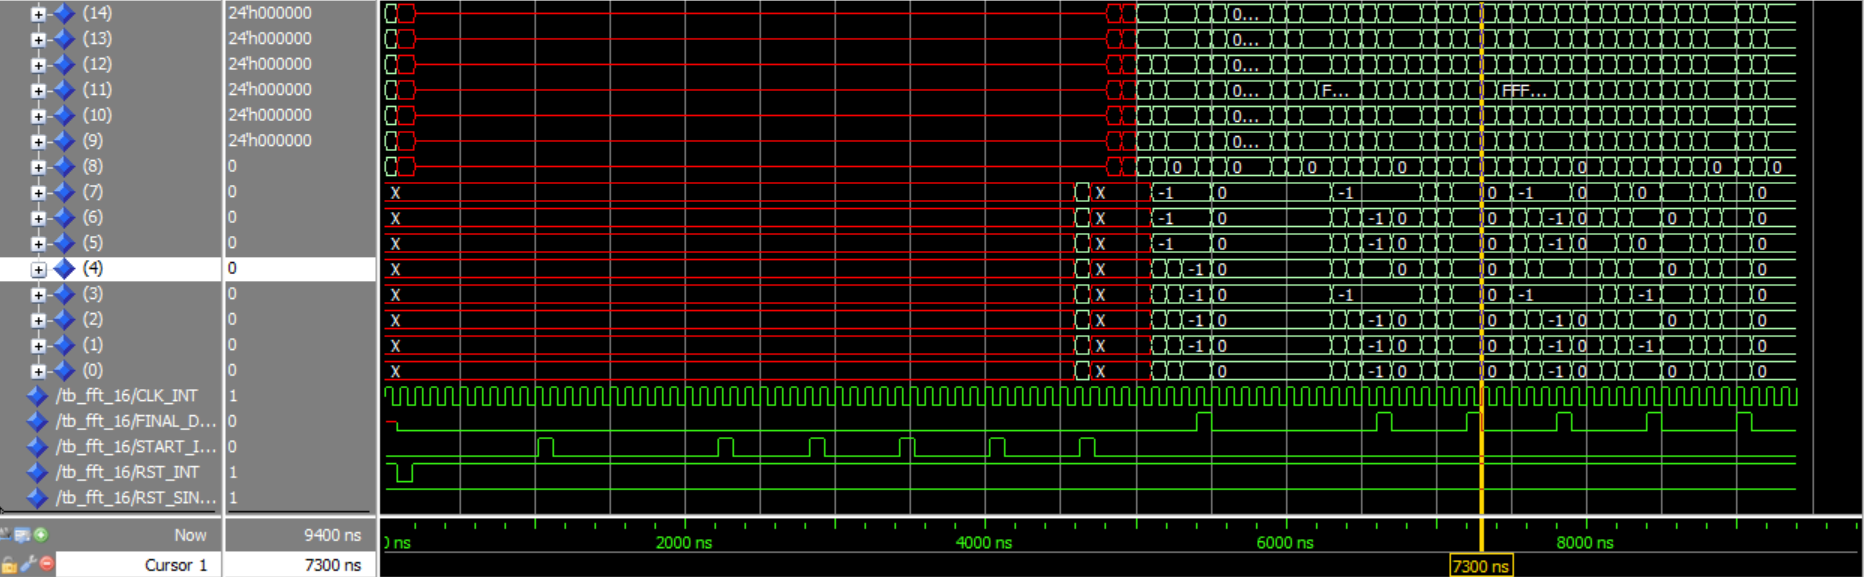
\includegraphics[width=1\textwidth]{sim_test3_imag}
      \caption{Schermata della simulazione completa, con focus sulle parti immaginarie dei risultati del test 3}
\end{figure}
\begin{figure}[H]
      \centering
      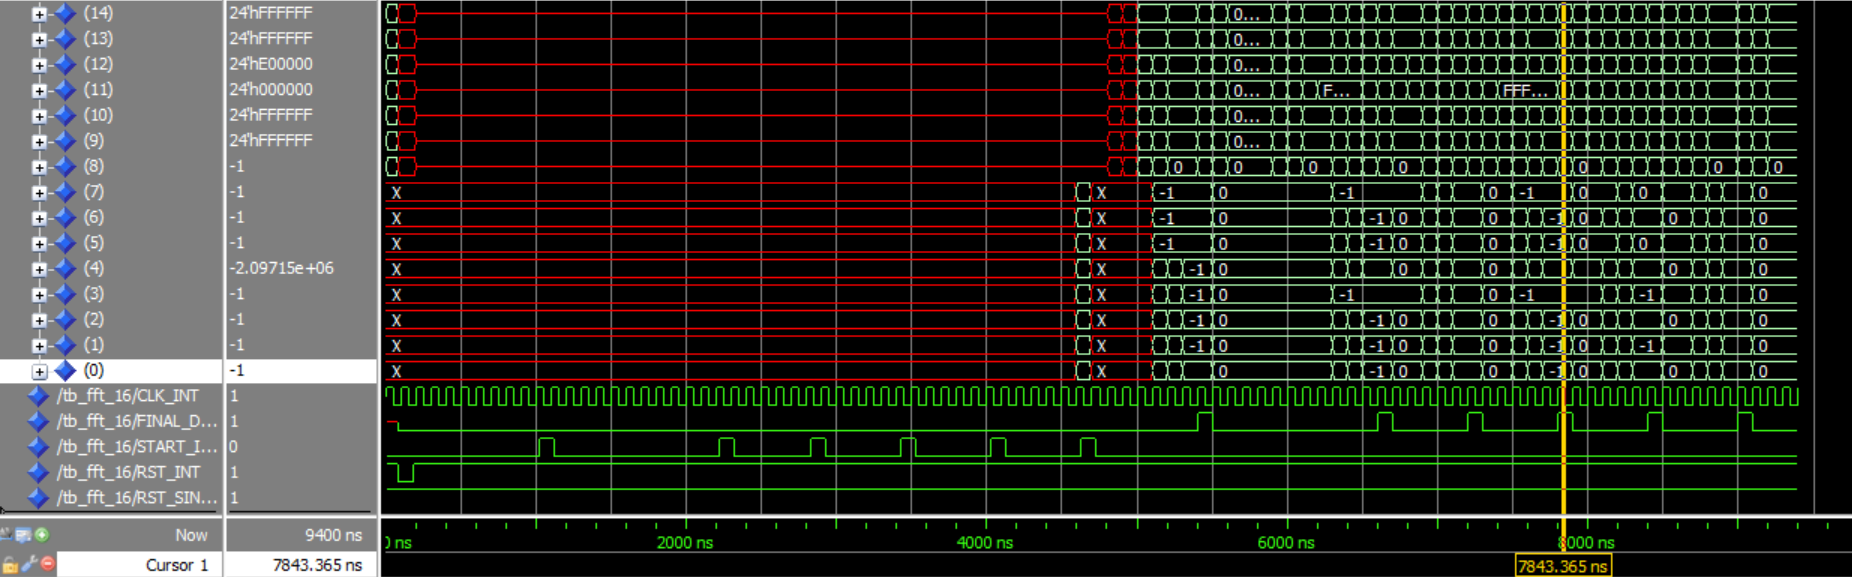
\includegraphics[width=1\textwidth]{sim_test4_real}
      \caption{Schermata della simulazione completa, con focus sulle parti reali dei risultati del test 4}
\end{figure}
\begin{figure}[H]
      \centering
      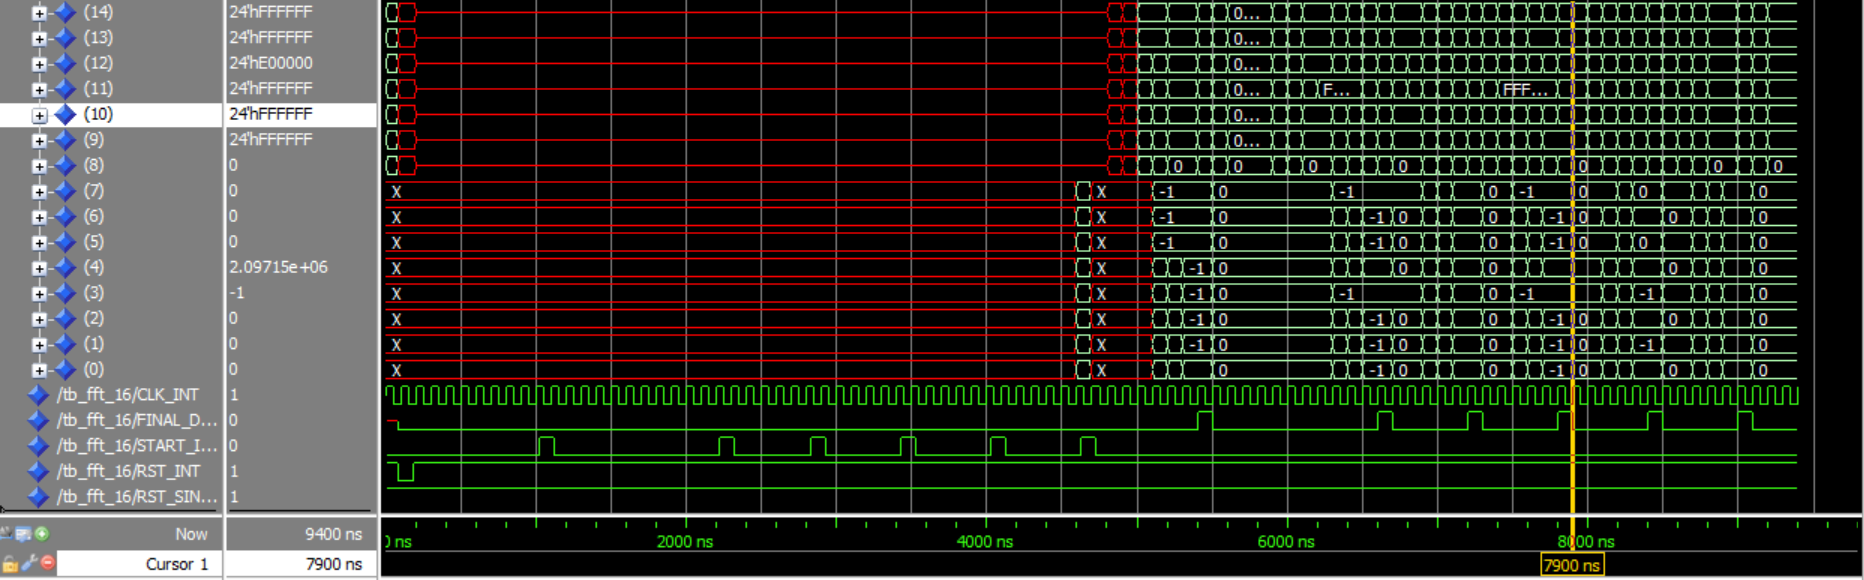
\includegraphics[width=1\textwidth]{sim_test4_imag}
      \caption{Schermata della simulazione completa, con focus sulle parti immaginarie dei risultati del test 4}
\end{figure}
\begin{figure}[H]
      \centering
      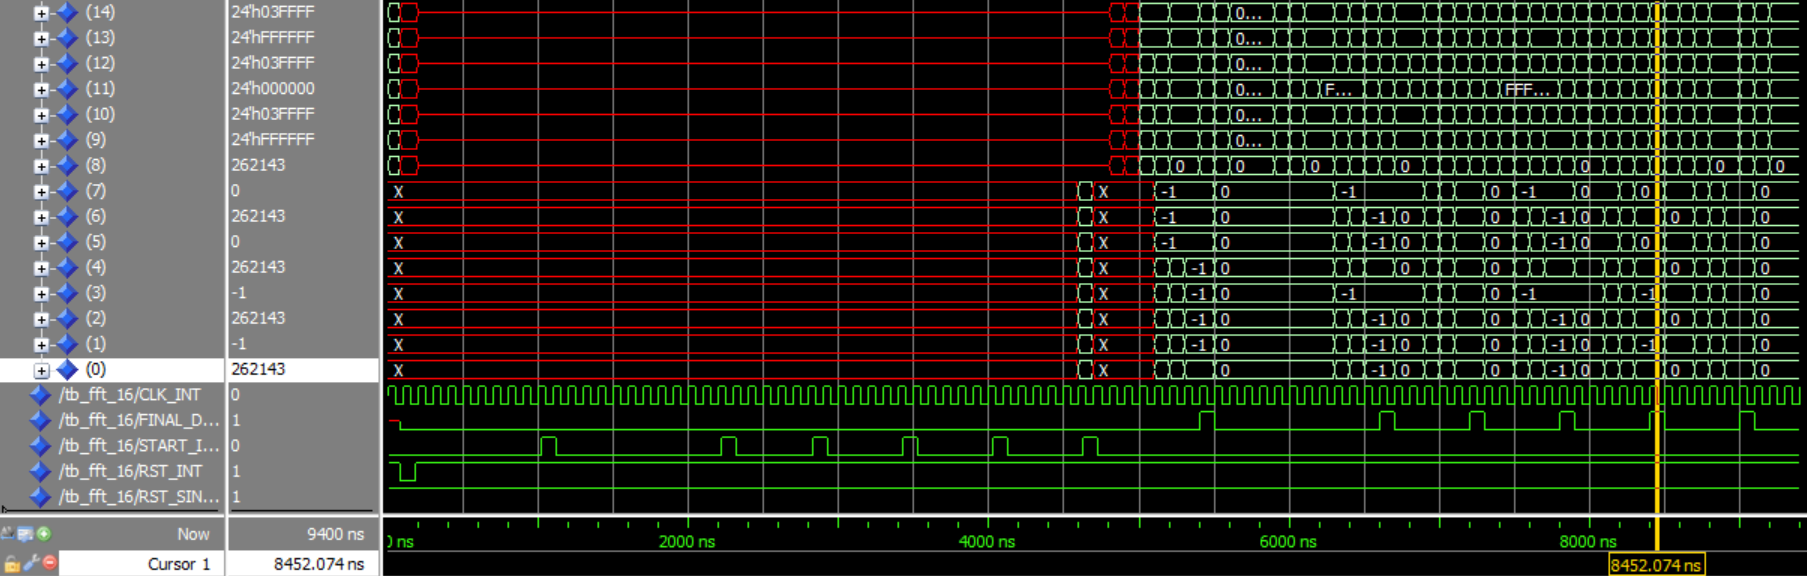
\includegraphics[width=1\textwidth]{sim_test5_real}
      \caption{Schermata della simulazione completa, con focus sulle parti reali dei risultati del test 5}
\end{figure}
\begin{figure}[H]
      \centering
      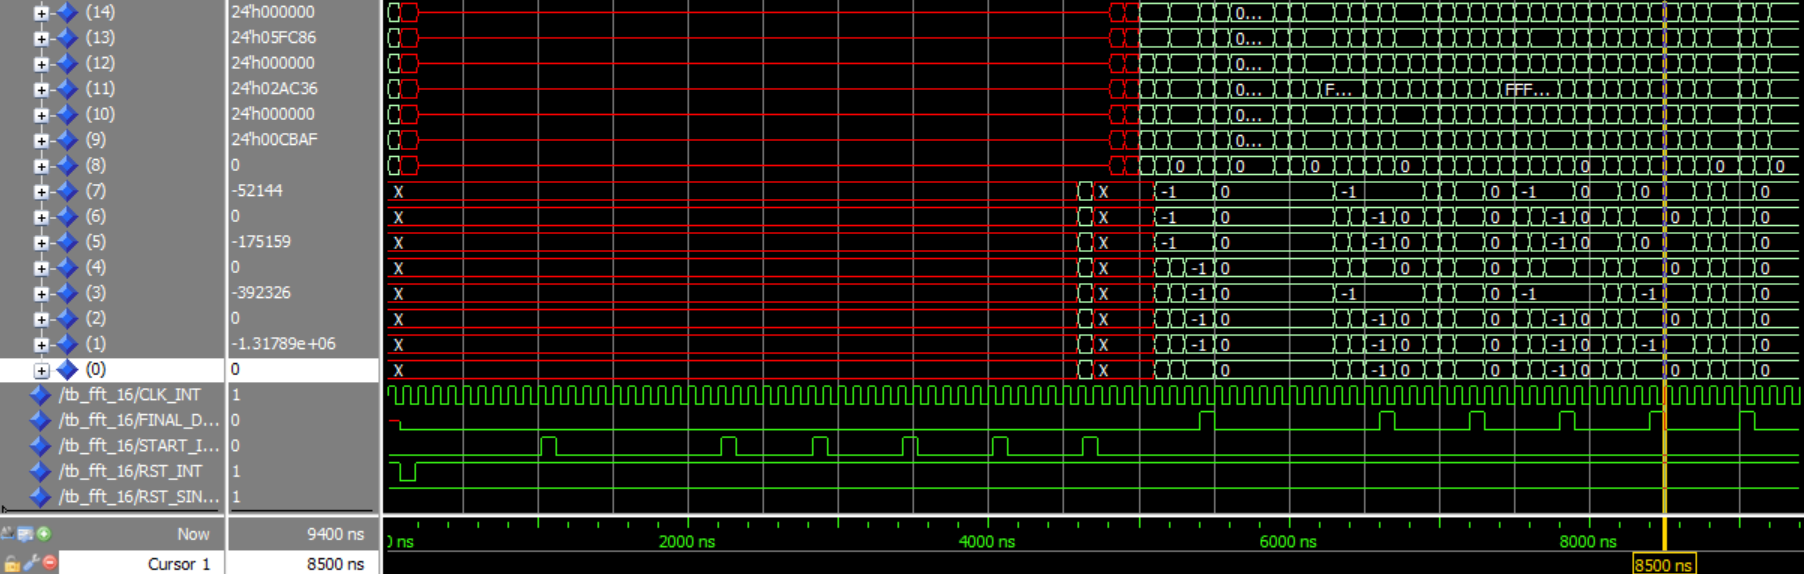
\includegraphics[width=1\textwidth]{sim_test5_imag}
      \caption{Schermata della simulazione completa, con focus sulle parti immaginarie dei risultati del test 5}
\end{figure}
\begin{figure}[H]
      \centering
      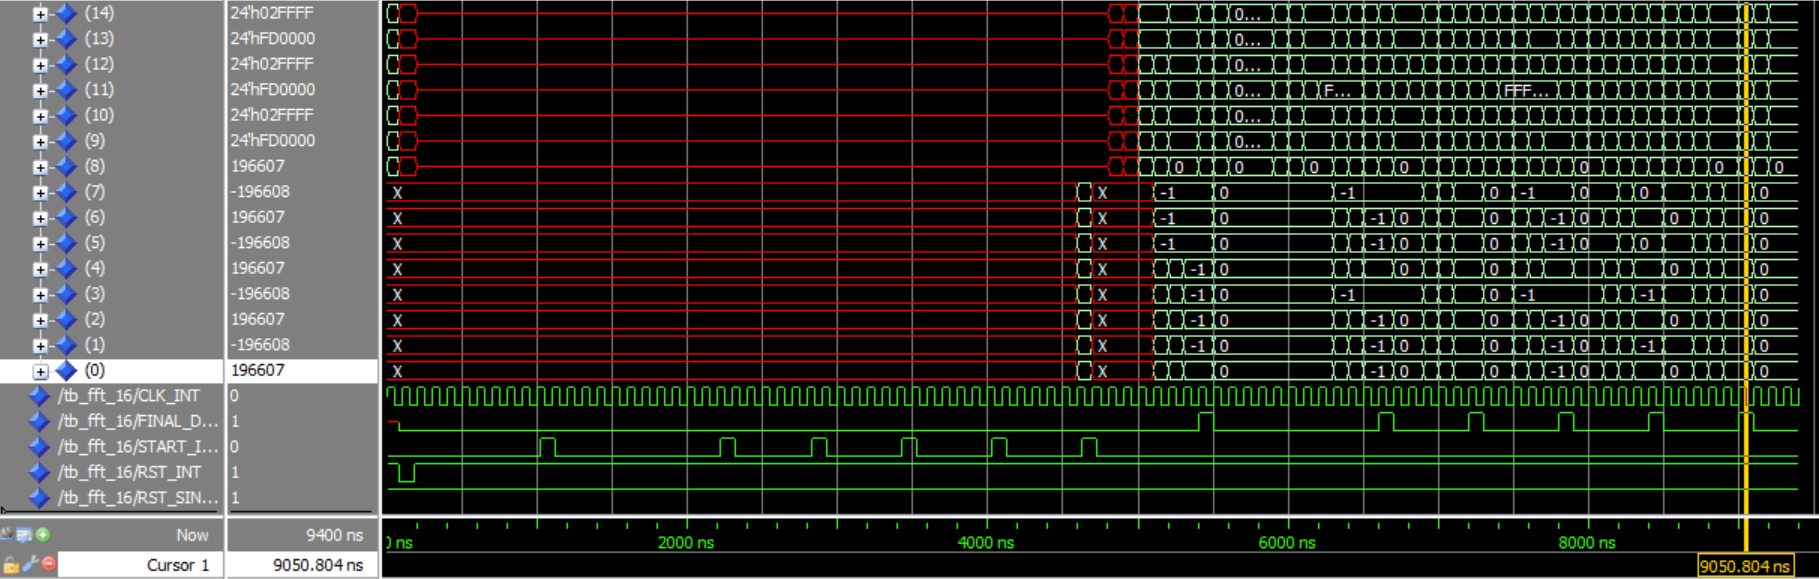
\includegraphics[width=1\textwidth]{sim_test6_real}
      \caption{Schermata della simulazione completa, con focus sulle parti reali dei risultati del test 6}
\end{figure}
\begin{figure}[H]
      \centering
      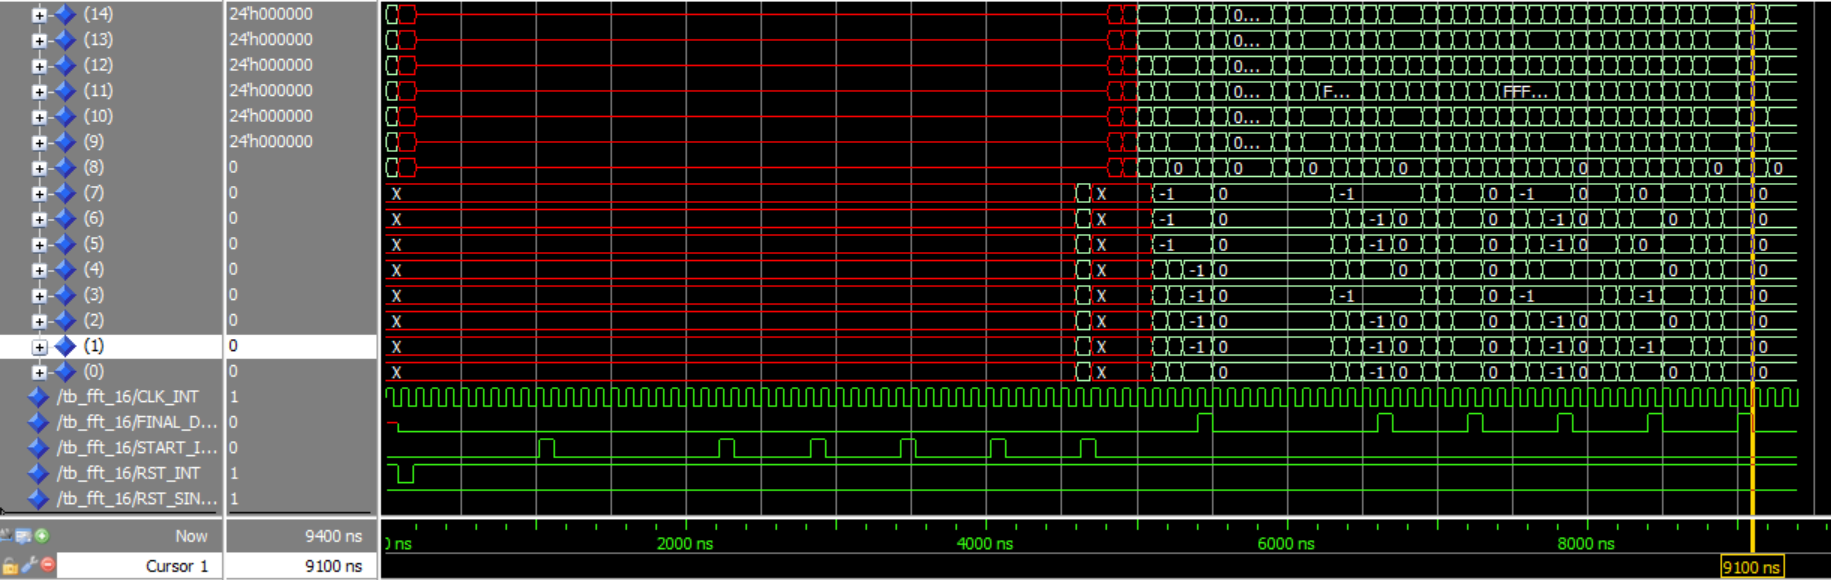
\includegraphics[width=1\textwidth]{sim_test6_imag}
      \caption{Schermata della simulazione completa, con focus sulle parti immaginarie dei risultati del test 6}
\end{figure}
\noindent Dalle schermate riportate della simulazione completa, in cui il periodo di clock è stato impostato a 100 ns, si sottolinea come gli output soddisfino i valori attesi dai sei test. Si osserva anche che il primo fronte di START avviene a 1100 ns e il relativo DONE (indicato come $FINAL\_DONE$) è alto in corrispondenza del fronte a 5500 ns. La differenza è esattamente 4400 ns, che è il tempo necessario per una butterfly a generare un segnale DONE (1100 ns rispetto al fronte di salita del clock in cui è attivo lo START relativo) moltiplicato per 4 (il numero di stadi). Perciò, come atteso, la latenza di una singola butterfly risulta essere pari a 12 periodi di clock (poi le parti immaginarie vengono fornite in uscita il colpo successivo all'attivazione del done), mentre la latenza di ogni FFT è di 45 colpi di clock. Inoltre, si osserva che, nonostante la latenza sia la medesima sia in modalità continua che in modalità singola, nel primo caso genero un segnale di DONE (e quindi risultati validi) ogni 6 colpi di clock.

\noindent A seguire, si riportano le tabelle in cui vengono confrontati i risultati aspettati con quelli ottenuti dalla simulazione, tenendo conto che, per rapportare correttamente i valori espressi come signed forniti in ambito simulativo con le uscite attese, è necessario convertirli in fixed point, dividendo per $2^{23}$, e moltiplicarli per lo scale factor, pari a 32. I dati ottenuti risultano essere estremamente precisi e in accordo con i risultati attesi, anche per via del ridotto numero di cifre significative dei risultati con cui si è effettuata la comparazione.

\begin{table}[H]
\centering
\resizebox{\textwidth}{!}{% % Forza la tabella a stare nella larghezza del testo
\begin{tabular}{|c|c|c|c|c|c|c|}
\hline
\textit{Indice} & \begin{tabular}[c]{@{}c@{}}\textit{parte reale}\\\textit{attesa}\end{tabular} & \begin{tabular}[c]{@{}c@{}}\textit{parte immaginaria}\\\textit{attesa}\end{tabular} & \begin{tabular}[c]{@{}c@{}}\textit{parte reale}\\\textit{da simulaz.}\end{tabular} & \begin{tabular}[c]{@{}c@{}}\textit{parte immaginaria}\\\textit{da simulaz.}\end{tabular} & \begin{tabular}[c]{@{}c@{}}\textit{parte reale}\\\textit{scalata}\end{tabular} & \begin{tabular}[c]{@{}c@{}}\textit{parte immaginaria}\\\textit{scalata}\end{tabular} \\ \hline
0 & -16 & 0 & -4.1943e+06 & 0 & $\approx$ -15.99998 & 0 \\ \hline
1 & 0 & 0 & -1 & 0 & $\approx$ -3.8e-06 & 0 \\ \hline
2 & 0 & 0 & -1 & 0 & $\approx$ -3.8e-06 & 0 \\ \hline
3 & 0 & 0 & -1 & 0 & $\approx$ -3.8e-06 & 0 \\ \hline
4 & 0 & 0 & -1 & 0 & $\approx$ -3.8e-06 & 0 \\ \hline
5 & 0 & 0 & -1 & 0 & $\approx$ -3.8e-06 & 0 \\ \hline
6 & 0 & 0 & -1 & 0 & $\approx$ -3.8e-06 & 0 \\ \hline
7 & 0 & 0 & -1 & 0 & $\approx$ -3.8e-06 & 0 \\ \hline
8 & 0 & 0 & -1 & 0 & $\approx$ -3.8e-06 & 0 \\ \hline
\end{tabular}%
}
\caption{Tabella riassuntiva per il vettore di test 1}
\end{table}

\begin{table}[H]
\centering
\resizebox{\textwidth}{!}{% % Adatta la tabella alla larghezza della pagina
\begin{tabular}{|c|c|c|c|c|c|c|}
\hline
\textit{Indice} & \begin{tabular}[c]{@{}c@{}}\textit{parte reale}\\\textit{attesa}\end{tabular} & \begin{tabular}[c]{@{}c@{}}\textit{parte immaginaria}\\\textit{attesa}\end{tabular} & \begin{tabular}[c]{@{}c@{}}\textit{parte reale}\\\textit{da simulaz.}\end{tabular} & \begin{tabular}[c]{@{}c@{}}\textit{parte immaginaria}\\\textit{da simulaz.}\end{tabular} & \begin{tabular}[c]{@{}c@{}}\textit{parte reale}\\\textit{scalata}\end{tabular} & \begin{tabular}[c]{@{}c@{}}\textit{parte immaginaria}\\\textit{scalata}\end{tabular} \\ \hline
0 & 0 & 0 & -1 & 0 & $\approx$ -3.8e-06 & 0 \\ \hline
1 & 0 & 0 & -1 & 0 & $\approx$ -3.8e-06 & 0 \\ \hline
2 & 0 & 0 & -1 & 0 & $\approx$ -3.8e-06 & 0 \\ \hline
3 & 0 & 0 & -1 & -1 & $\approx$ -3.8e-06 & $\approx$ -3.8e-06  \\ \hline
4 & -8 & 0 & -2.09715e+06 & 0 & $\approx$ -7.999992 & 0 \\ \hline
5 & 0 & 0 & -1 & 0 & $\approx$ -3.8e-06 & 0 \\ \hline
6 & 0 & 0 & -1 & 0 & $\approx$ -3.8e-06 & 0 \\ \hline
7 & 0 & 0 & -1 & -1 & $\approx$ -3.8e-06 & $\approx$ -3.8e-06  \\ \hline
8 & 0 & 0 & -1 & 0 & $\approx$ -3.8e-06 & 0 \\ \hline
\end{tabular}%
}
\caption{Tabella riassuntiva per il vettore di test 2}
\end{table}

\begin{table}[H]
\centering
\resizebox{\textwidth}{!}{% % Adatta la tabella alla larghezza della pagina
\begin{tabular}{|c|c|c|c|c|c|c|}
\hline
\textit{Indice} & \begin{tabular}[c]{@{}c@{}}\textit{parte reale}\\\textit{attesa}\end{tabular} & \begin{tabular}[c]{@{}c@{}}\textit{parte immaginaria}\\\textit{attesa}\end{tabular} & \begin{tabular}[c]{@{}c@{}}\textit{parte reale}\\\textit{da simulaz.}\end{tabular} & \begin{tabular}[c]{@{}c@{}}\textit{parte immaginaria}\\\textit{da simulaz.}\end{tabular} & \begin{tabular}[c]{@{}c@{}}\textit{parte reale}\\\textit{scalata}\end{tabular} & \begin{tabular}[c]{@{}c@{}}\textit{parte immaginaria}\\\textit{scalata}\end{tabular} \\ \hline
0 & 1 & 0 & 262143 & 0 & $\approx$ 0.999996 & 0 \\ \hline
1 & 1 & 0 & 262143 & 0 & $\approx$ 0.999996 & 0 \\ \hline
2 & 1 & 0 & 262143 & 0 & $\approx$ 0.999996 & 0 \\ \hline
3 & 1 & 0 & 262143 & 0 & $\approx$ 0.999996 & 0 \\ \hline
4 & 1 & 0 & 262143 & 0 & $\approx$ 0.999996 & 0 \\ \hline
5 & 1 & 0 & 262143 & 0 & $\approx$ 0.999996 & 0 \\ \hline
6 & 1 & 0 & 262143 & 0 & $\approx$ 0.999996 & 0 \\ \hline
7 & 1 & 0 & 262143 & 0 & $\approx$ 0.999996 & 0 \\ \hline
8 & 1 & 0 & 262143 & 0 & $\approx$ 0.999996 & 0 \\ \hline
\end{tabular}%
}
\caption{Tabella riassuntiva per il vettore di test 3}
\end{table}

\begin{table}[H]
\centering
\resizebox{\textwidth}{!}{% % Adatta la tabella alla larghezza della pagina
\begin{tabular}{|c|c|c|c|c|c|c|}
\hline
\textit{Indice} & \begin{tabular}[c]{@{}c@{}}\textit{parte reale}\\\textit{attesa}\end{tabular} & \begin{tabular}[c]{@{}c@{}}\textit{parte immaginaria}\\\textit{attesa}\end{tabular} & \begin{tabular}[c]{@{}c@{}}\textit{parte reale}\\\textit{da simulaz.}\end{tabular} & \begin{tabular}[c]{@{}c@{}}\textit{parte immaginaria}\\\textit{da simulaz.}\end{tabular} & \begin{tabular}[c]{@{}c@{}}\textit{parte reale}\\\textit{scalata}\end{tabular} & \begin{tabular}[c]{@{}c@{}}\textit{parte immaginaria}\\\textit{scalata}\end{tabular} \\ \hline
0 & 0 & 0 & -1 & 0 & $\approx$ -3.8e-06 & 0 \\ \hline
1 & 0 & 0 & -1 & 0 & $\approx$ -3.8e-06 & 0 \\ \hline
2 & 0 & 0 & -1 & 0 & $\approx$ -3.8e-06 & 0 \\ \hline
3 & 0 & 0 & -1 & -1 & $\approx$ -3.8e-06 & $\approx$ -3.8e-06 \\ \hline
4 & -8 & 8 & -2.09715e+06 & 2.09715e+06 & $\approx$ -7.999992 & $\approx$ +7.999992 \\ \hline
5 & 0 & 0 & -1 & 0 & $\approx$ -3.8e-06 & 0 \\ \hline
6 & 0 & 0 & -1 & 0 & $\approx$ -3.8e-06 & 0 \\ \hline
7 & 0 & 0 & -1 & 0 & $\approx$ -3.8e-06 & 0 \\ \hline
8 & 0 & 0 & -1 & 0 & $\approx$ -3.8e-06 & 0 \\ \hline
\end{tabular}%
}
\caption{Tabella riassuntiva per il vettore di test 4}
\end{table}

\begin{table}[H]
\centering
\resizebox{\textwidth}{!}{% % Adatta la tabella alla larghezza della pagina
\begin{tabular}{|c|c|c|c|c|c|c|}
\hline
\textit{Indice} & \begin{tabular}[c]{@{}c@{}}\textit{parte reale}\\\textit{attesa}\end{tabular} & \begin{tabular}[c]{@{}c@{}}\textit{parte immaginaria}\\\textit{attesa}\end{tabular} & \begin{tabular}[c]{@{}c@{}}\textit{parte reale}\\\textit{da simulaz.}\end{tabular} & \begin{tabular}[c]{@{}c@{}}\textit{parte immaginaria}\\\textit{da simulaz.}\end{tabular} & \begin{tabular}[c]{@{}c@{}}\textit{parte reale}\\\textit{scalata}\end{tabular} & \begin{tabular}[c]{@{}c@{}}\textit{parte immaginaria}\\\textit{scalata}\end{tabular} \\ \hline
0 & 1 & 0 & 262143 & 0 & $\approx$ 0.999996 & 0 \\ \hline
1 & 0 & -5.027 & -1 & -1.31789e+06 & $\approx$ -3.8e-06 & $\approx$ -5.027 \\ \hline
2 & 1 & 0 & 262143 & 0 & $\approx$ 0.999996 & 0 \\ \hline
3 & 0 & -1.497 & -1 & -392326 & $\approx$ -3.8e-06 & $\approx$ -1.497 \\ \hline
4 & 1 & 0 & 262143 & 0 & $\approx$ 0.999996 & 0 \\ \hline
5 & 0 & -0.668 & 0 & -175159 & 0 & $\approx$ -0.668 \\ \hline
6 & 1 & 0 & 262143 & 0 & $\approx$ 0.999996 & 0 \\ \hline
7 & 0 & -0.199 & 0 & -52144 & 0 & $\approx$ -0.199 \\ \hline
8 & 1 & 0 & 262143 & 0 & $\approx$ 0.999996 & 0 \\ \hline
\end{tabular}%
}
\caption{Tabella riassuntiva per il vettore di test 5}
\end{table}


\begin{table}[H]
\centering
\resizebox{\textwidth}{!}{% % Adatta la tabella alla larghezza della pagina
\begin{tabular}{|c|c|c|c|c|c|c|}
\hline
\textit{Indice} & \begin{tabular}[c]{@{}c@{}}\textit{parte reale}\\\textit{attesa}\end{tabular} & \begin{tabular}[c]{@{}c@{}}\textit{parte immaginaria}\\\textit{attesa}\end{tabular} & \begin{tabular}[c]{@{}c@{}}\textit{parte reale}\\\textit{da simulaz.}\end{tabular} & \begin{tabular}[c]{@{}c@{}}\textit{parte immaginaria}\\\textit{da simulaz.}\end{tabular} & \begin{tabular}[c]{@{}c@{}}\textit{parte reale}\\\textit{scalata}\end{tabular} & \begin{tabular}[c]{@{}c@{}}\textit{parte immaginaria}\\\textit{scalata}\end{tabular} \\ \hline
0 & 0.75 & 0 & 196607 & 0 & $\approx$ 0.749996 & 0 \\ \hline
1 & -0.75 & 0 & -196608 & 0 &  -0.75 & 0 \\ \hline
2 & 0.75 & 0 & 196607 & 0 & $\approx$ 0.749996 & 0 \\ \hline
3 & -0.75 & 0 & -196608 & 0 &  -0.75 & 0 \\ \hline
4 & 0.75 & 0 & 196607 & 0 & $\approx$ 0.749996 & 0 \\ \hline
5 & -0.75 & 0 & -196608 & 0 &  -0.75 & 0 \\ \hline
6 & 0.75 & 0 & 196607 & 0 & $\approx$ 0.749996 & 0 \\ \hline
7 & -0.75 & 0 & -196608 & 0 &  -0.75 & 0 \\ \hline
8 & 0.75 & 0 & 196607 & 0 & $\approx$ 0.749996 & 0 \\ \hline
\end{tabular}%
}
\caption{Tabella riassuntiva per il vettore di test 6}
\end{table}


\noindent Infine, si riporta lo screenshot di una simulazione dedicata, che mostra l'effetto del Reset Sincrono (indicato come RST\_SINC\_INT); successivamente all'attivazione di tale segnale, come descritto nella sottosezione \ref{subsec:reset}, tutte le butterfly presenti nell'architettura vengono riportate allo stato di IDLE. Infatti,  è possibile notare come, nonostante siano stati inviati correttamente 7 segnali di START, si trasmettono in uscita dalla FFT solo cinque segnali di DONE attivi; poiché la terza e la quarta elaborazione richiesta dei dati in ingresso non è ancora terminata quando viene richiesto un reset della macchina.


\begin{figure}[H]
      \centering
      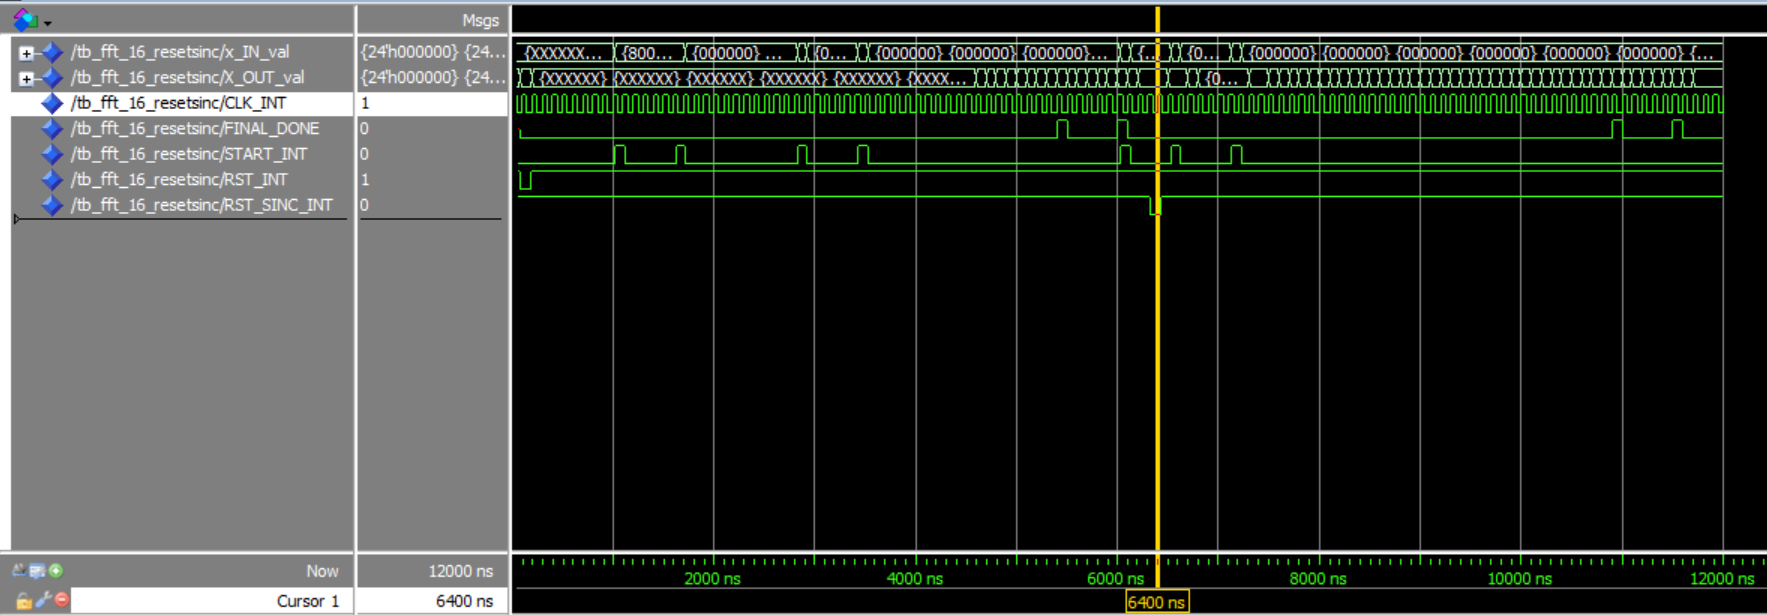
\includegraphics[width=1\textwidth]{sim_reset_sinc}
      \caption{Schermata della simulazione completa, con focus sul Reset Sincrono}
\end{figure}
